\documentclass[11pt,a4paper]{article}
\usepackage[T1]{fontenc}
\usepackage[utf8]{inputenc}
\usepackage{lmodern,microtype,graphicx,booktabs,longtable,tabularx,array,amsmath,amssymb}
\usepackage[margin=22mm]{geometry}
\usepackage[colorlinks=true,linkcolor=black,citecolor=black,urlcolor=blue]{hyperref}
\usepackage[numbers,sort&compress]{natbib}
\widowpenalty=10000
\clubpenalty=10000
\setlength{\parskip}{4pt}
\setlength{\parindent}{12pt}
\setlength{\emergencystretch}{2em}
\renewcommand{\thesection}{S\arabic{section}}
\renewcommand{\thetable}{S\arabic{table}}
\renewcommand{\theequation}{S\arabic{equation}}
\title{Supporting Information\\[0.5em]\large An agentic framework for X-ray absorption spectroscopy of catalytic interfaces}
\author{Haili Jia and Maria K. Y. Chan\\[0.5em]
\small Center for Nanoscale Materials, Argonne National Laboratory,\\
\small 9700 South Cass Avenue, Lemont, Illinois 60439, United States\\
\small Corresponding author: \href{mailto:mchan@anl.gov}{mchan@anl.gov}}
\hypersetup{pdftitle={Supporting Information for An agentic framework for X-ray absorption spectroscopy of catalytic interfaces},pdfauthor={Haili Jia and Maria K. Y. Chan}}
\date{}
\usepackage{pdflscape}
\renewcommand{\thefigure}{S\arabic{figure}}
\begin{document}
\maketitle
\noindent Sections S1--S7 preserve the frozen 87-configuration study and its historical evidence. The new source-corrected paired study is defined separately below; its records do not overwrite that snapshot.
\section{Interface construction and structural labels}
The lateral interface construction represents two distinct fcc metals with matching (111) facets. Metal identities and row counts define the ordered stripe geometry. Adsorption regions distinguish boundary rows, nearby rows, and terrace regions. Available placement controls include single-binding adsorbates, multidentate species, and coupled carbon-containing intermediates. The broader Cu--Au sampling plan includes 1:1, 2:1, 1:2, 3:1, and 1:3 stripe ratios as well as pure-metal reference surfaces. These ratios describe the construction space; they do not imply that every parent or adsorbate combination is present in the completed spectral cohort.

Molecular atom correspondence is retained through relaxation. Chemical labels distinguish the requested intermediate from the molecular components in the relaxed calculation structure. Initial molecule mappings are reconciled with the saved atom order, and local metal layers and contacts are refreshed after relaxation. Geometric screening considers short contacts, periodic images, molecular formulas, bonds and angles, unintended coupling between molecules, and placement relative to the surface. The general interface checker uses periodicity in the surface plane and a nonperiodic vacuum direction. Its distance rules are structural screening criteria rather than electronic bond-order or thermodynamic assignments.

The completed-dataset component analysis uses the C/O/H connectivity in the actual structure used for spectral calculation. Pair cutoffs are 1.85, 1.70, 1.30, 1.20, 0.90, and 1.65~\AA{} for C--C, C--O, C--H, O--H, H--H, and O--O, respectively. Verified molecular identities require compatible bond graphs, not elemental composition alone. An OCCO assignment requires a C--C bond, two C--O bonds, no O--O bond, and the corresponding carbon and oxygen degrees. The position of hydrogen distinguishes CHO from COH and COCHO from OCCOH. Assignments must remain unchanged when cutoffs are scaled by 0.9 and 1.1; ambiguous components are retained for review rather than used as identity targets. The shared audit uses in-plane minimum images and a nonperiodic vacuum direction. The reported primary predictions remain those of the archived cohort.

For species $s$, molecular coverage is $N_s/N_{\rm ref}$, where $N_{\rm ref}$ is the declared surface reference population. The reference and molecular counts are retained separately from the number of occupied metal sites. For OCCO plus spectator CO, carbon-equivalent coverage is
\begin{equation}
\theta_{\rm C}=(2N_{\rm OCCO}+N_{\rm CO})/N_{\rm ref}.
\end{equation}
Thus two CO molecules and one OCCO molecule can have equal carbon loading but different molecular coverages. Coadsorbed species are represented by simultaneous species-presence labels. COCO is a legacy alias of the bonded OCCO construction template; the unbonded comparator is denoted 2CO. Observed connectivity determines the relaxed-state label.

\section{Electronic-structure and spectral calculations}
Structural relaxation is performed with VASP.\cite{vasp1996} The committed Cu--Au relaxation examples use a 520~eV plane-wave cutoff, electronic convergence of $10^{-5}$~eV, a force threshold of 0.05~eV~\AA$^{-1}$, fixed cell vectors, and a $\Gamma$-centered $1\times1\times1$ mesh. The adjacent-CO example fixes the bottom three metal layers and relaxes the top two. A dipole correction is applied normal to the asymmetric slab. These are input-example parameters; the completed-cohort records retain the available per-calculation settings.

The present inference dataset uses FDMNES Green-function multiple-scattering calculations.\cite{joly2001} Parsed settings for the representative CO configurations include self-consistency, a 6.0~\AA{} cluster radius, the Perdew option, photon-energy output, and a relative energy range of $-5$ to $50$~eV in 0.2~eV steps. The recorded convolved spectra span 8974.0--9029.0~eV with 276 points. Available record fields do not independently specify every core-hole or broadening parameter. The spectra analyzed here are the saved convolved outputs; no new broadening or energy alignment was fitted during model evaluation.

The archived layer inputs contain SCF, Green, and Perdew keywords but no explicit SCFexc, Screening, nohole, or Gamma\_hole setting. The output banners identify a 28 July 2026 program revision. The available user guide describes a ground-state self-consistent calculation without a core hole at the K edge, followed by introduction of the hole and screening charge for the absorption calculation.\cite{fdmnesmanual} This is an inference from the inputs and documented defaults, not an explicitly recorded core-hole specification; the available guide is dated November 2022. Of the 348 layer spectra, 332 have separate convolution logs reporting Gamma\_hole = 1.55~eV and Gamma\_max = 10~eV; the other 16 do not have separate convolution logs. These settings therefore cannot be asserted from logs for every layer. A matching guide or source revision is unavailable, so the core-hole prescription is not treated as independently established for that executable. The benchmark reference logs instead identify 11 April 2025 and must not be substituted for the ML-cohort logs.

The framework also generates FEFF and VASP spectroscopy inputs.\cite{rehr2010,vaspxas} Shared structural linkage does not imply identical absorber populations or equivalent numerical approximations between backends. The numerical inference scores in the main paper concern FDMNES Cu K-edge data only. Carbon and oxygen edges and other backends form separate potential comparison channels.

\section{Data quality and absorber-population checks}
The source inventory contains 172 locations and 155 unique physical structures. Identical source geometries are counted once, including when multiple directories refer to the same structure. Calculation copies within site or layer folders are not counted as new independent configurations. For the full inventory, an unreadable or empty relaxed-structure file can be replaced by a readable initial structure; its presence does not establish a completed relaxation.

A completed spectral record must provide finite, nonconstant Cu K-edge arrays for layers 2--5 on compatible energy grids. Layer ordering is checked against absorber heights, the physical top Cu sites, and the position of adsorbates. Spectral arrays are compared with their saved convolved output, while coordinates, element identities, and atom indices are checked against the relaxed simulation structure. The six FDMNES lattice parameters are reconciled with the relaxed cell before coordinates are compared in a common frame; matching fractional coordinates alone is insufficient. Length and angle tolerances are $2\times10^{-5}$~\AA{} and $2\times10^{-5}$ degrees, respectively. Records with inconsistent chemical identities or unresolved molecular assignments are not accepted as training labels.

The final convolution population is reconciled with the layer absorber table. This is necessary because a completed directory can include both full-layer calculations and later subset calculations. In two CO configurations, the final convolution represents 36 sites although subset main inputs or intermediate logs describe three sites. Full-population assignment was established by matching the final convolution contributions to their raw spectra, using an energy-cutoff tolerance of approximately 0.00051~eV, complete atom coverage, and compatible grids. These cases are included. A separate CO configuration with an incompatible layer-5 grid is excluded.

Seven records required corrections to molecular identities, counts, or site-species labels. Measurements were unchanged. Duplicate geometries and identical complete spectral stacks were removed before cross-validation. Table~\ref{tab:cohort} summarizes the resulting cohort.

\begin{table}[htbp]\centering
\caption{Dataset accounting.}\label{tab:cohort}
\begin{tabular}{@{}lr@{}}\toprule
Quantity & Count\\\midrule
Source locations &172\\
Unique inventory structures &155\\
Completed-record files &102\\
Duplicate records removed &14\\
Grid-incompatible record excluded &1\\
Independent configurations retained &87\\
Layer spectra retained &348\\
Mixed-species configurations &9\\
Single-species configurations &78\\\bottomrule
\end{tabular}
\end{table}

\section{Spectral population weighting and feature construction}
Let $\mu_l(E)$ denote the raw mean cross section for a layer containing $n_l$ represented Cu sites. Before normalization, the spectrum for a chosen set $D$ of layers is
\begin{equation}
\mu_D(E)=\frac{\sum_{l\in D}n_l\mu_l(E)}{\sum_{l\in D}n_l}.
\end{equation}
The seven fixed-depth representations are the four individual layers and averages over the top two, top three, and four available layers. The last representation excludes the unsampled bottom layer and contains no additional attenuation or detection-mode weighting.

For each representation, the minimum intensity is subtracted and the result is normalized by its integrated area. Feature families are: normalized intensity on the recorded energy grid; cumulative trapezoidal integral; first derivative; concatenated smoothed shape, cumulative integral, first derivative, and second derivative; and the first 24 type-II orthonormal discrete-cosine coefficients. Savitzky--Golay smoothing and derivatives use an 11-point window with a third-order polynomial and the energy-grid spacing. The area and transformations are calculated separately for each sample.

Using $\widetilde\mu(E)$ for the minimum-subtracted, unit-area-normalized spectrum, the figure labels correspond to
\begin{align}
\mathrm{Norm}_k &= \widetilde\mu(E_k),\\
\mathrm{CDF}_k &= \int_{E_{\min}}^{E_k}\widetilde\mu(E)\,\mathrm dE,\\
\mathrm{d1}_k &= \left.\frac{\mathrm d\widetilde\mu}{\mathrm dE}\right|_{E_k}.
\end{align}
The numerical derivative uses the stated Savitzky--Golay polynomial fit. Combined concatenates the Savitzky--Golay-smoothed normalized spectrum, CDF, d1, and the second derivative. DCT24 contains coefficients $c_0,\ldots,c_{23}$ of the type-II orthonormal discrete cosine transform of the normalized spectrum; the zero-frequency coefficient is included. The transform follows the type-II cosine basis.\cite{ahmed1974} The 24 retained coefficients are a fixed representation dimension in the candidate set, rather than an independently optimized physical cutoff. For $N$ energy samples $x_j=\widetilde\mu(E_j)$, the coefficients are \begin{equation}
c_k=\alpha_k\sum_{j=0}^{N-1}x_j\cos\!\left[\frac{\pi k(2j+1)}{2N}\right],\qquad
\alpha_0=N^{-1/2},\quad \alpha_{k>0}=\sqrt{2/N},\quad k=0,\ldots,23.
\end{equation}
The representations are alternative numerical views of each spectrum, not additional independent samples.


Additional tree candidates use multiscale spectrum/derivative channels with windows of 7, 11, and 21 points, or the surface spectrum together with a surface-minus-subsurface contrast. The latter channels share the sample's surface-area normalization to preserve relative depth amplitudes. No molecular count, site label, geometry descriptor, or filename is used as a spectral predictor.

\section{Models and nested evaluation}
The candidate set includes balanced logistic regression with $C=1$, an RBF SVM with $C=3$ and scale-dependent kernel width, multi-output random forests and extra-trees, and independent binary extra-trees for each species.\cite{geurts2006} Joint forests use 96 trees; the independent ensembles use 64 trees per species. Random forests use a minimum leaf size of two, while extra-trees use a leaf size of one. Both use square-root feature subsampling. Logistic regression and SVM inputs are standardized using statistics fitted on training data only. A sigmoid of the SVM decision function supplies a thresholdable score rather than a calibrated probability. Constant-label training partitions receive constant scores. PCA is not used in this benchmark.

Five outer folds hold out whole configurations with test sizes of 17, 17, 17, 18, and 18. The original assignments of 85 configurations are retained; two recovered configurations are allocated by label balance and fold size without using spectra or prediction results. Each configuration's four layers and combined-layer variants share the same fold. Three inner folds are drawn within each outer-training partition. Candidate inner assignments are ranked by the number of missing-positive training labels and label imbalance, using training labels alone. Fold assignments are supplied with the analysis outputs.

The primary selector compares independent-species tree representations and thresholds within each outer-training set. The global threshold candidates are 0.15, 0.25, 0.35, 0.45, 0.50, 0.55, 0.65, and 0.75. Guarded species-specific adjustments require at least five positive and ten negative training configurations. Adjustments are restricted to a neighborhood of the global threshold and shrunk halfway toward it; they are retained only when the training-fold selection objective improves. Micro F1 is the primary selection objective. The fixed-depth comparison restricts the candidate set to one depth representation while selecting its features and thresholds.

Micro F1 pools true positives, false positives, and false negatives across species. Macro F1 averages the species-level F1 values over all 11 observed species, including failures on rare labels. Exact identity-set accuracy requires the full predicted species set to match the reference. The independent selector gives micro/macro F1 of 0.779/0.638 and exact-set accuracy of 0.690. Table~\ref{tab:species} gives its species-level results.

\begin{table}[htbp]\centering\small
\caption{Primary selector by species. Counts are positive configurations and overlap for mixtures.}\label{tab:species}
\begin{tabular}{@{}lrrrr@{}}\toprule
Species & Positives & Precision & Recall & F1\\\midrule
CHO & 5 & 0.500 & 0.200 & 0.286\\
CO & 30 & 1.000 & 0.867 & 0.929\\
CO2 & 3 & 0.667 & 0.667 & 0.667\\
COCHO & 1 & 0.000 & 0.000 & 0.000\\
COH & 6 & 1.000 & 0.500 & 0.667\\
COOH & 8 & 0.714 & 0.625 & 0.667\\
H & 22 & 0.933 & 0.636 & 0.757\\
O & 7 & 1.000 & 0.714 & 0.833\\
OCCOH & 4 & 1.000 & 0.500 & 0.667\\
OCHO & 8 & 0.857 & 0.750 & 0.800\\
OH & 5 & 1.000 & 0.600 & 0.750\\
\bottomrule
\end{tabular}
\end{table}


The fixed extra-trees/first-derivative/surface combination has the highest observed score among the compared fixed entries: micro/macro F1 of 0.798/0.660 and exact-set accuracy of 0.701. This ranking uses outer-fold results and is exploratory. Repeated analysis of the same simulated cohort does not provide an external confirmation set.

Conditional 95\% intervals use 1500 bootstrap resamples of held-out configurations, with the fitted predictions held fixed. Paired depth differences use the same resampled configurations. The intervals exclude model-refitting uncertainty and are not corrected for multiple comparisons. The random seed is 20261020.

\section{Figure construction and structural comparisons}
All new figure elements are generated by the accompanying plotting code. The circular workflow uses vector graphics, and the substrate rendering in Figure 2a preserves the metal coordinates from the representative input, with adsorbates omitted from that view. The molecular gallery is shown separately, with one element legend shared by the whole panel. The archived coupling design preserves the supplied starting coordinates without modifying bond distances. The extended Cu--Au site diagram is an ideal triangular fcc(111) surface with explicitly specified metal identities, adsorbate positions, and site contacts. The Cu--Au bridge has one contact on each side of the indicated boundary. CuCuCu, CuCuAu, and CuAuAu hollows are defined by three explicit metal contacts. Surface and adsorbate coordinates share one oblique projection. Figure 2b assigns each adsorbate-bearing configuration to one single-species or coadsorbed bin; it omits two clean structures and one CuO reference. These schematic coordinates are supplied separately from the calculated input structures. The molecular gallery uses schematic geometries with explicitly declared bond graphs; these illustrations represent chemical connectivity rather than optimized bond lengths. All molecular drawings share the same coordinate scale and display radius for atomic symbols; these symbol sizes do not represent ionic or van der Waals radii.

The archived reference panels used reference-v2; the updated reference-v3 comparison is given below. The exact fixed-window 0--1 arrays feed both display and similarities; no separate maximum division or earlier edge-jump scores are mixed with them. No graphical display paths are used for metrics. The layer-resolved panel uses recorded CO spectral arrays. The previous species-present/absent descriptive contrast is omitted from the main figure because its reference contains other adsorbates and cannot isolate an adsorbate-induced change. Its historical arrays are retained for provenance only, not as a clean control.

The carbon-coupling figure uses four actual starting models containing two C and two O atoms. Minimum input C--C distances are approximately 2.52~\AA{} for adjacent CO at the Cu-side interface, 2.46~\AA{} for adjacent CO on the Cu terrace, and 1.45~\AA{} for both OCCO models. These distances are not relaxed bond lengths. A matched spectral test requires the same parent, loading, numerical settings, and absorber-population definitions, together with verified final connectivity. No eligible intact-OCCO positives occur in the current inference cohort.


\section{Reproduction and software integration}
The archived held-out predictions and reported tables can be replayed without refitting. A separate natural-language-agent run invoked the archived primary selector on a relocated, byte-hashed 87-configuration export and rebuilt 895 fit-cache entries. It reproduced the primary micro/macro F1 of 0.7791/0.6383 and exact identity-set accuracy of 0.6897. Primary and exploratory-winner prediction arrays matched the archive. Across the broader comparison, 140 of 169 held-out array files matched exactly; 29 differed, predominantly in logistic-regression and support-vector variants, with differences also in some random-forest and macro-selected outputs. The rerun used NumPy 2.4.6 and scikit-learn 1.9.0, compared with archived versions 2.3.5 and 1.8.0. These differences are consistent with dependency sensitivity but do not isolate its cause. The archive was not overwritten. All five newly saved outer-fold models reproduced their held-out predictions after reload. This repeats the original cohort and does not constitute independent confirmation.

The agent and graphical interface call a shared audited-training route. Its archived-primary option is distinct from a separate global-threshold integration recipe. A local execution fixture links simulated scheduler events, a saved relaxed geometry, an existing FDMNES record, and held-out model inference. It tests software handoffs; it does not establish production scheduler execution or generation of new spectra.

The full-cohort export contains the relaxed coordinates, spectral records, absorber tables, calculation inputs and outputs, final convolution evidence, frozen folds, and correction provenance needed to repeat the audit and fitting. Byte hashes protect its link to the archived protocol. Figure-only reproduction uses the accompanying plotted data and requires neither model fitting nor access to the simulation tree. Both modes preserve the distinction between the primary nested selector and the exploratory fixed winner.

The training-most-common-set baseline is fitted separately in each outer-training partition and gives micro/macro F1 of 0.323/0.047 and exact-set accuracy of 0.241. The training-majority binary baseline predicts no species and gives zero for all three measures. All baseline results use the frozen configuration folds.


\clearpage
\section{Source-resolved reconstruction and corrected records}
The new audit uses 116 usable completed configurations (99 Cu--Au and 17 Cu(100)), with two physical top layers each. All 232 native final convolutions are reproduced from saved electronic source spectra and original decks. Source hashes, header multiplicities, physical atom indices, $E_{\rm cut}$, $E_{\rm psii}$, shifts, generated decks and numerical residuals are retained per layer. Twenty-eight layers have nonunit source multiplicities, including the clean interface and seven adsorbed Cu--Au configurations. The aggregate source multiplicity is not a physical atom count.

The raw site cross-section is symmetry summed. Where the convolution source list already includes every physical Cu atom, the corrected per-Cu signal is
\begin{equation}
\mu_l(E)=\frac{1}{N_l}\,\mathcal{C}\left[\sum_{j\in l}\frac{x_j(E)}{m_j}\right],
\end{equation}
where $m_j$ is the recorded source multiplicity and $\mathcal{C}$ retains the original source-specific energy convention and final convolution prescription. Explicit unit-weight controls reproduce the native implicit source sum. Inverse-multiplicity weights recover one contribution per physical absorber. This is an audited source convention, not inference from atom-count uniqueness alone. Layers without nonunit multiplicities retain their original scale.

The uploaded reconstruction tool is an October 22, 2026 official FDMNES package; its hashes and source URL are pinned. The saved electronic outputs identify July 28, 2026. Numerical reproduction of the convolution does not prove that later source documents the earlier electronic core-hole default. Core-hole metadata therefore remain \texttt{not\_reported}; the historical 332/348 separate broadening logs are not silently extended to the 16 missing logs. No new electronic spectrum or HPC job is generated.
\begin{figure}[!htbp]\centering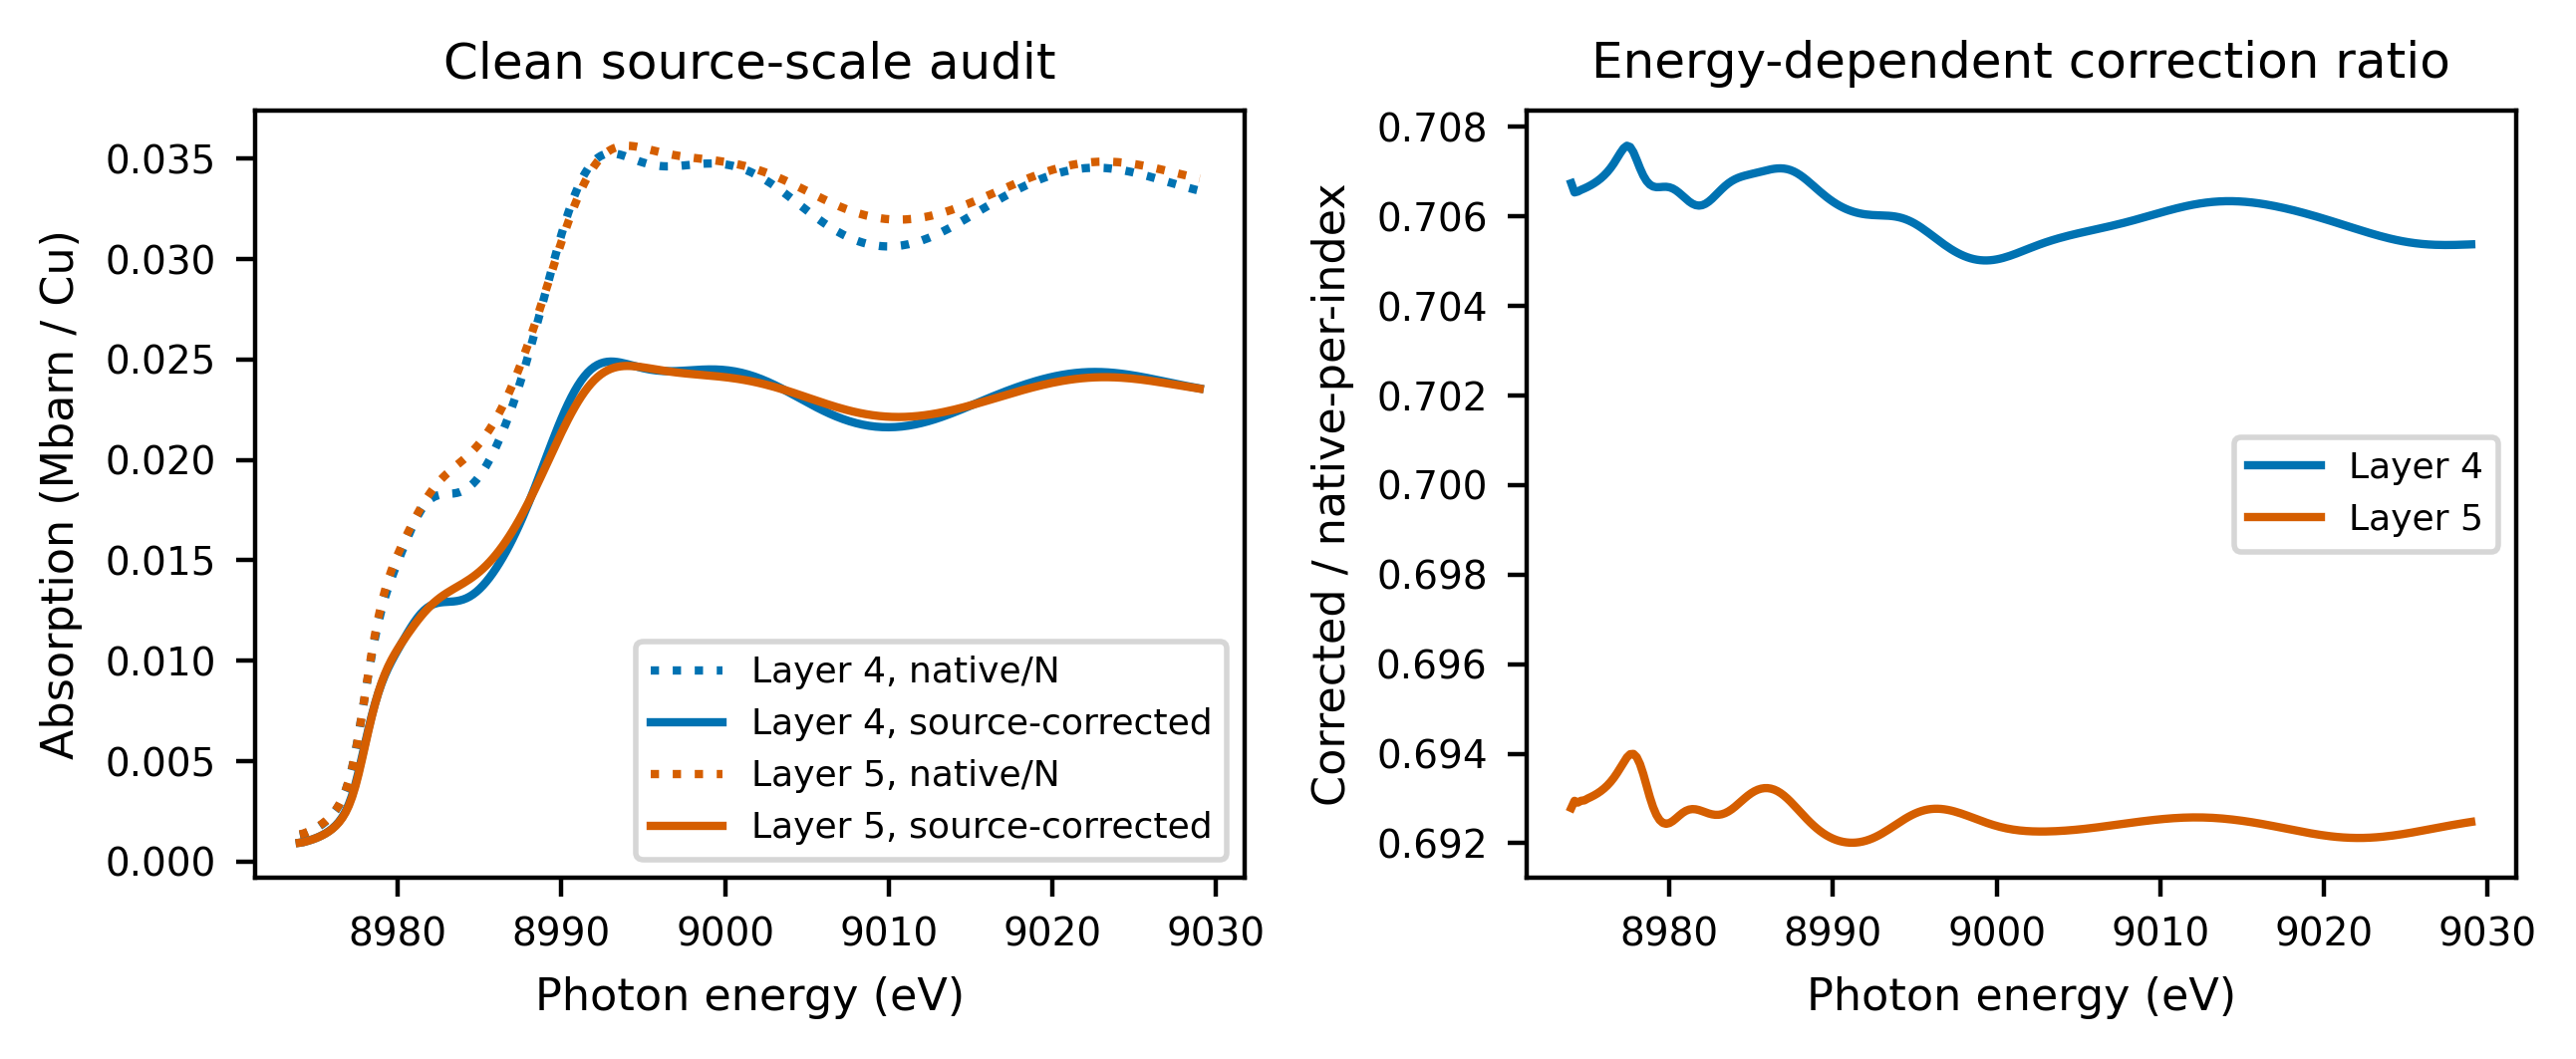
\includegraphics[width=\linewidth]{figures/SI_source_scale.png}
\caption{Native aggregate divided by unique atom count versus source-corrected physical per-Cu spectra for the actual clean reference. The ratio varies with energy, precluding correction by a guessed scalar. Dotted lines denote native-per-index; solid lines denote source-resolved correction.}\end{figure}

\section{Pair definitions, signed features and units}
The primary 34 cases have identical initial metal coordinates, cell, composition and constraints to the clean model; this is strong model compatibility, without independently proven historic ancestry. Sixty-four weaker same-substrate/model cases are kept separate. The pair manifest records paths, SHA-256, energy support, physical populations, settings, observed labels, matching evidence and exclusion status. One clean-model family serves all eligible pairs; 66 distinct metal-coordinate arrangements are not asserted to be independent parent families. No matched OCHO support is inferred from a same-cell reference.

The common supported grid is 8974--9029 eV in 0.2 eV steps, with linear interpolation and no extrapolation. Physical Cu--Au populations are 36 per layer in layers 4+5; Cu(100) uses four per layer in 3+4. The top-two combination uses population weights in both members. No Cu(100) clean reference is substituted from Cu--Au, bulk Cu, or an adsorbate-bearing state. Raw electronic and final convolution sources are retained separately. The clean edge-step windows are 8974--8977 and 9018--9025 eV, using one shared divisor for every pair member. No fitted pairwise alignment is applied.

Let $d_j=\Delta\mu(E_j)/S$ and $h=0.2$ eV. The signed-grid representation contains $d_j$. A fixed Savitzky--Golay smoother has 11 points and polynomial degree 3; its first and second derivatives use $h$ explicitly, giving units $S^{-1}\mu$/eV and $S^{-1}\mu$/eV$^2$. The cumulative difference is
\begin{equation}
 C_j=\sum_{k=1}^{j}\frac{d_{k-1}+d_k}{2}(E_k-E_{k-1}),\qquad C_0=0.
\end{equation}
It has relative-intensity eV units and may decrease. It is not a probability CDF. Combined concatenates smoothed signed intensity, cumulative difference and both derivatives. Training-only feature scaling does not rescale a query's amplitude independently.

For $N$ grid points, orthonormal type-II DCT coefficients are
\begin{equation}
 c_k=\alpha_k\sum_{j=0}^{N-1}d_j\cos\!\left[\frac{\pi}{N}\left(j+\frac12\right)k\right],\quad
 \alpha_0=N^{-1/2},\quad\alpha_{k>0}=\sqrt{2/N}.
\end{equation}
DCT8/16/24 retain $k=0,\ldots,K-1$, including DC.\cite{ahmed1974} No per-sample amplitude normalization follows the transform. Unit tests independently check analytic cumulative integrals, linear amplitude response, self-subtraction zero, both signs, DC, incompatible-reference rejection and shared-gain calibration.
\begin{figure}[!htbp]\centering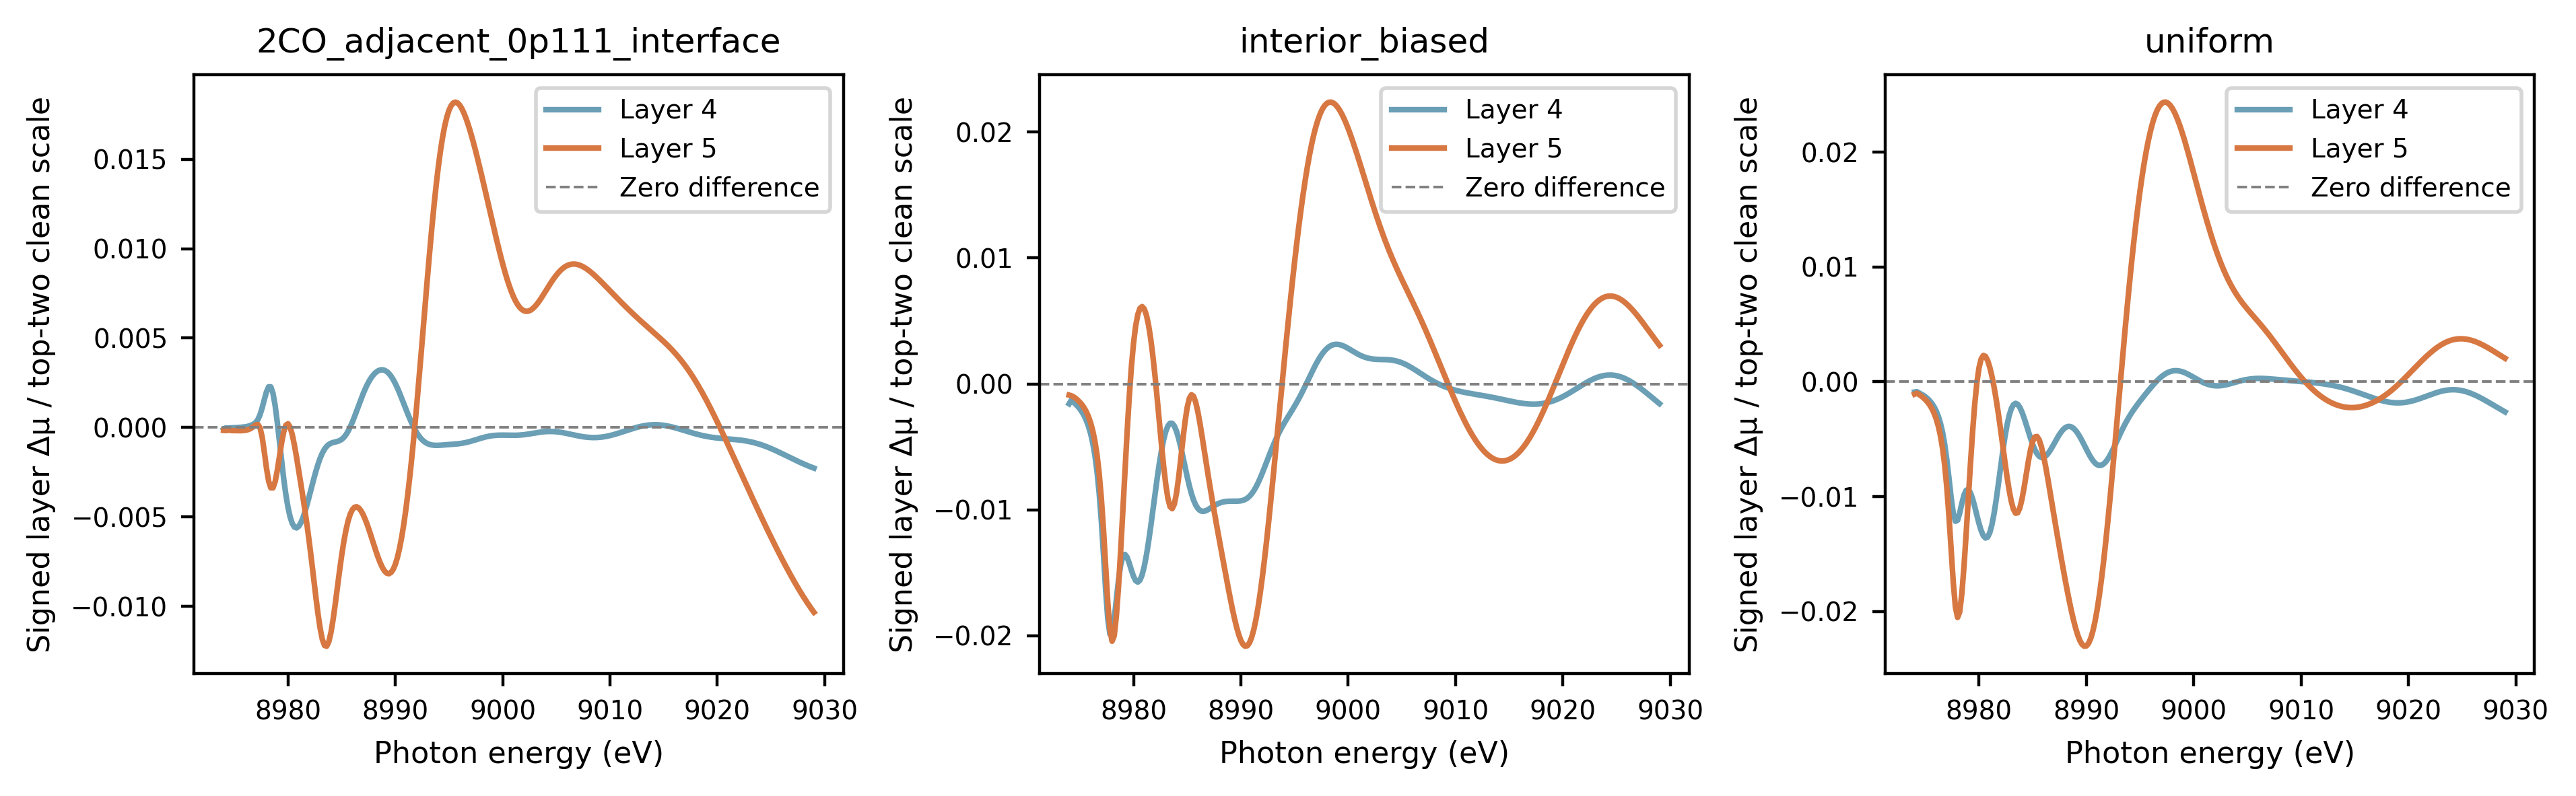
\includegraphics[width=\linewidth]{figures/SI_layer_differences.png}
\caption{Layer-resolved actual paired differences for the three equal-loading examples in the main text. The same top-two clean scale is used for both layers; their individual amplitudes are not renormalized. Dashed gray lines denote zero.}\end{figure}

\section{New grouped evaluation and complete score tables}
\begin{sloppypar}
Outer GroupKFold(5) partitions configurations; inner GroupKFold(3) selects Combined/DCT8/16/24 and compact regularization.\\ Regression candidates are Ridge $\alpha=1,10,100$ and two leaf-size-2 tree controls. Identity uses independent balanced logistic classifiers with $C=0.1,1$ and two compact tree controls. Single-class outer or inner training labels use constant predictions. Inner predictions set per-label thresholds; no outer test label selects features, regularization or thresholds. Nearly constant columns are removed using training data before feature scaling. This prevents constant clean-reference padding from changing random feature selection. All layer/absorber views remain with the configuration. No structural targets enter predictors.
\end{sloppypar}

The five representations are compared on identical matched cohorts, and the 98-case weaker reference set is a separate sensitivity study. The fixed one-reference affine control gives equivalent predictions for raw, difference and clean-plus-difference inputs. Per-species supports, scores, every selected recipe and inner prediction array accompany the saved outer predictions and models. The six primary supported labels are CO, H, O, COH, COOH and OH; macro scores over all eleven targets are not interpreted as support for absent chemistry.

\begingroup\footnotesize\setlength{\tabcolsep}{3pt}
\begin{longtable}{lllll}
\caption{Identity on identical configurations within each declared cohort.}\\
\toprule
Scope & Input & Micro F1 & Macro F1 (11) & Exact set\\\midrule\endfirsthead
Scope & Input & Micro F1 & Macro F1 (11) & Exact set\\\midrule\endhead
matched & legacy norm. & 0.7385 & 0.3259 & 0.6471\\
matched & corrected norm. & 0.7463 & 0.3375 & 0.6471\\
matched & per-Cu raw & 0.7941 & 0.3635 & 0.6765\\
matched & delta & 0.7941 & 0.3635 & 0.6765\\
matched & paired & 0.7941 & 0.3635 & 0.6765\\
matched & training\_label\_majority & 0.0000 & 0.0000 & 0.0000\\
weaker & legacy norm. & 0.6759 & 0.5584 & 0.5306\\
weaker & corrected norm. & 0.7109 & 0.5622 & 0.6020\\
weaker & per-Cu raw & 0.7426 & 0.6072 & 0.6224\\
weaker & delta & 0.7426 & 0.6072 & 0.6224\\
weaker & paired & 0.7426 & 0.6072 & 0.6224\\
weaker & training\_label\_majority & 0.0000 & 0.0000 & 0.0000\\
\bottomrule\end{longtable}\endgroup

\begingroup\footnotesize\setlength{\tabcolsep}{3pt}
\begin{longtable}{lllll}
\caption{CO-only loading relative to all surface metal sites; primary seven cases, weaker-reference sensitivity 25 cases. Missing or negative predictive value is retained.}\\
\toprule
Scope & Input & MAE & RMSE & $R^2$\\\midrule\endfirsthead
Scope & Input & MAE & RMSE & $R^2$\\\midrule\endhead
matched & legacy norm. & 0.0069 & 0.0098 & 0.6715\\
matched & corrected norm. & 0.0076 & 0.0103 & 0.6348\\
matched & per-Cu raw & 0.0065 & 0.0091 & 0.7143\\
matched & delta & 0.0065 & 0.0091 & 0.7143\\
matched & paired & 0.0065 & 0.0091 & 0.7143\\
matched & train mean & 0.0169 & 0.0212 & -0.5396\\
weaker & legacy norm. & 0.0144 & 0.0232 & 0.9318\\
weaker & corrected norm. & 0.0146 & 0.0240 & 0.9270\\
weaker & per-Cu raw & 0.0140 & 0.0237 & 0.9288\\
weaker & delta & 0.0140 & 0.0237 & 0.9288\\
weaker & paired & 0.0140 & 0.0237 & 0.9288\\
weaker & train mean & 0.0658 & 0.0930 & -0.0967\\
\bottomrule\end{longtable}\endgroup

An explicit mixture diagnostic applies the mean of the five saved CO-only fold models to four matched CO-containing mixture configurations, absent from every model fit and selection. Physical raw and differential MAE is 0.02021 CO/all surface metal sites, with $R^2=-10.31$. Thus the CO-only predictor does not establish mixture coverage inference; coadsorbates change the spectral response. This frozen-model diagnostic is distinct from mixture-trained cross-validation.

\begin{center}\small\begin{tabular}{lrr}\toprule
Input & Matched mixtures (4) MAE & Weaker mixtures (12) MAE\\\midrule
Legacy normalized & 0.01878 & 0.02221\\
Corrected normalized & 0.01972 & 0.02326\\
Physical raw & 0.02021 & 0.02546\\
Signed difference & 0.02021 & 0.02546\\
Paired & 0.02021 & 0.02546\\
\bottomrule\end{tabular}\end{center}
Conditional paired intervals resample configurations 1000 times with seed 20261027. They condition on fixed predictions and do not measure refitting, parent transfer or a prospective test. Repeated use of the existing folds is exploratory. A new fit is not independent confirmation. Configuration-level geometry targets are evaluated separately using fixed DCT16/Ridge(10); primary contact targets are constant, and broader hollow compositions lack CuAu$_2$/Au$_3$ support. Molecular support cannot inflate the configuration sample count.

\section{Cu(100), missing controls and domain scope}
The raw loading control fixes DCT16/StandardScaler/Ridge(10) and the original grouped Cu--Au folds. Four Cu(100) CO configurations use leave-one-configuration-out augmentation with the other three, while a Cu--Au-only control sees none. Targets are CO/surface Cu loading. It reproduces the four previously reported MAEs without changing target denominators. The separate raw identity control uses CO/H/O/OH only, fixed DCT16/balanced logistic $C=1$ and inner grouped thresholds. Twelve Cu(100) configurations have these supported labels; five H$_2$O/CO$_3$ cases are explicit unsupported chemistry, and carbonate connectivity does not establish charge. Domain-balanced summaries must use domain-level scores rather than counting the larger domain as independent transfer evidence.

No completed compatible clean Cu(100) run was located in the current CO2RR, original Cu-Ox updated structures/100, Cu100 exports, Downloads or unpacked source roots. The prepared Cu16 clean seed is derived from the original parent by removing adsorbates; it is a proposed relaxation input, not an already relaxed reference or completed frozen-metal calculation. Bottom layers are fixed and top layers are free. A guard requires successful ionic relaxation before complete top-layer XAS decks are generated. No jobs were submitted. Joint differential training and unseen-parent validation remain unavailable until this control and adequate independent families exist.

\section{Synthetic robustness protocol and physical interpretation}
All stress settings are fixed before examining outer results. Shared rigid energy errors are $\pm0.2,0.5,1,2$ eV; residual reference-only errors are $\pm0.2,0.5,1$ eV. Shared recalibrated gains, relative adsorbate gain and edge-step errors are $\pm2,5\%$. Extra Gaussian $\sigma=0.25,0.5,1$ eV uses a positive normalized finite-domain kernel; native lifetime broadening remains. Independent Gaussian noise amplitudes are 1, 2 and 5\% of peak intensity, with three seeds. Shared-reference scenarios reuse the same reference noise realization across query configurations, retaining dependency. This simplified pointwise noise is not an instrument model.

Both pair members are perturbed before subtraction. The fixed interior grid 8976--9027 eV supports every shift without extrapolation. Raw and difference controls use identical cropped grids and outer folds. The compact fixed stress model is DCT16/Ridge(10) for coverage or independent balanced logistic $C=1$ for identity; thresholds use inner grouped folds. Training-only augmentation uses four deterministic views with shared shifts $-0.5,-0.2,0.2,0.5$ eV, relative shift $\pm0.2$ eV, 1\% gain/noise and Gaussian $\sigma=0.25$ eV. Copies never cross folds; no stress curve selects nuisance settings. All 832 metric rows and corresponding held-out arrays are retained.

The stable-background dilution test uses $a_{\rm obs}=b+f(a-b)$ with $f=0.1,0.25,0.5,1$. It reports error against full surface loading and against the response proxy $f\theta$ separately. Neither determines the unknown illuminated surface fraction. Simulated top-two slab spectra do not establish experimental depth weighting. Experimental queries require independently documented per-Cu calibration, shared reference-derived edge-step windows, detection geometry, incident-intensity, thickness/concentration and self-absorption corrections, residual reference coverage, common energy calibration and an independent surface fraction. Without those, reference-free inference fails rather than borrowing a cross-facet mean reference. No paired labeled experimental accuracy is reported.\cite{ramaker2010,ramaker2014}

\section{Reference benchmark: processing order and complete similarities}
The preserved original notebook uses Gaussian $\sigma=1$ eV and exploratory $+120/+125$ eV shifts; one cell reuses a previous intensity variable, so its empty/unverified inputs cannot silently define a new curve. The new executed notebook records its actual arrays and corrected portable route. Raw $\rightarrow$ native output $\rightarrow$ fixed additional Gaussian (VASP only) $\rightarrow$ rigid alignment $\rightarrow$ common-grid min--max normalization are saved independently. Original experimental negative noise and native raw values remain unchanged; unsupported local pre-edge subtraction is removed before display normalization. Min--max scaling is relative intensity, not a cure for a faulty baseline.

Cu-calibrated offsets are fitted separately for every declared method, including PBE and the GW-labelled dataset. The shape diagnostic uses the first resolved Cu/Cu$_2$O peak and the early CuO inflection, not an arbitrary later peak. First-feature matching has no fitted width; Gaussian $\sigma=1$ eV is the notebook prescription rather than measured resolution. The feature search windows, nominal offsets, detected features, support checks and failure status are saved. No label-based outer-model result determines these windows. Chemical-shift accuracy is not inferred from per-compound shape alignment. Cu$_2$O FEFF retains common Cu calibration because its first feature is unresolved.

All scores and main plotted arrays use 176 points over 8980--9015 eV. Each trace, including experiment, uses identical-window extrema in $(I-I_{\min})/(I_{\max}-I_{\min})$. Flat/invalid traces and inadequate support are unavailable, not zero similarity. Cosine is $x\cdot y/(\|x\|\|y\|)$ without centering. Pearson correlates centered intensities; Spearman correlates ranks with ties. Official SciPy functions supply the correlations; no pointwise p-values imply independent energy samples. A high correlation cannot validate absolute energy, chemical shifts or a mechanism.

\begingroup\footnotesize\setlength{\tabcolsep}{3pt}
\begin{longtable}{lllllll}
\caption{Complete available reference similarities. Shift sign is $E_{photon}=E_{native}+shift$. CuO PBE has no valid numeric table and remains missing in both views.}\\
\toprule
Material & Method & View & Shift/eV & Cosine & $r$ & $\rho$\\\midrule\endfirsthead
Material & Method & View & Shift/eV & Cosine & $r$ & $\rho$\\\midrule\endhead
Cu & Green & Cu-cal. & 0.0452 & 0.9972 & 0.9852 & 0.9329\\
Cu & FDM & Cu-cal. & 3.0452 & 0.9908 & 0.9828 & 0.9313\\
Cu & FEFF & Cu-cal. & -7.7208 & 0.9874 & 0.9665 & 0.9619\\
Cu & PBE & Cu-cal. & 124.7218 & 0.9156 & 0.7413 & 0.5417\\
Cu & GW label & Cu-cal. & 125.0649 & 0.9779 & 0.8777 & 0.9593\\
Cu & Green & feature & 0.0452 & 0.9972 & 0.9852 & 0.9329\\
Cu & FDM & feature & 3.0452 & 0.9908 & 0.9828 & 0.9313\\
Cu & FEFF & feature & -7.7208 & 0.9874 & 0.9665 & 0.9619\\
Cu & PBE & feature & 124.7218 & 0.9156 & 0.7413 & 0.5417\\
Cu & GW label & feature & 125.0649 & 0.9779 & 0.8777 & 0.9593\\
Cu2O & Green & Cu-cal. & 0.0452 & 0.9953 & 0.9790 & 0.9355\\
Cu2O & FDM & Cu-cal. & 3.0452 & 0.9807 & 0.8645 & 0.7164\\
Cu2O & FEFF & Cu-cal. & -7.7208 & 0.9869 & 0.9099 & 0.7331\\
Cu2O & PBE & Cu-cal. & 124.7218 & 0.8975 & 0.6472 & 0.3493\\
Cu2O & GW label & Cu-cal. & 125.0649 & 0.8960 & 0.6469 & 0.7382\\
Cu2O & Green & feature & 0.2919 & 0.9963 & 0.9776 & 0.9390\\
Cu2O & FDM & feature & -0.7081 & 0.9978 & 0.9825 & 0.9711\\
Cu2O & FEFF & feature & -7.7208 & 0.9869 & 0.9099 & 0.7331\\
Cu2O & PBE & feature & 115.9511 & 0.9032 & 0.6446 & 0.7491\\
Cu2O & GW label & feature & 125.5837 & 0.9050 & 0.6627 & 0.7443\\
CuO & Green & Cu-cal. & 0.0452 & 0.9967 & 0.9754 & 0.8925\\
CuO & FDM & Cu-cal. & 3.0452 & 0.9468 & 0.8010 & 0.8326\\
CuO & FEFF & Cu-cal. & -7.7208 & 0.9872 & 0.9026 & 0.7954\\
CuO & GW label & Cu-cal. & 125.0649 & 0.9602 & 0.7940 & 0.7994\\
CuO & Green & feature & 0.8926 & 0.9963 & 0.9811 & 0.9107\\
CuO & FDM & feature & -0.5074 & 0.9607 & 0.7718 & 0.6316\\
CuO & FEFF & feature & -6.8164 & 0.9918 & 0.9437 & 0.8597\\
CuO & GW label & feature & 125.2560 & 0.9614 & 0.8073 & 0.8225\\
\bottomrule\end{longtable}\endgroup

\begin{figure}[p]\centering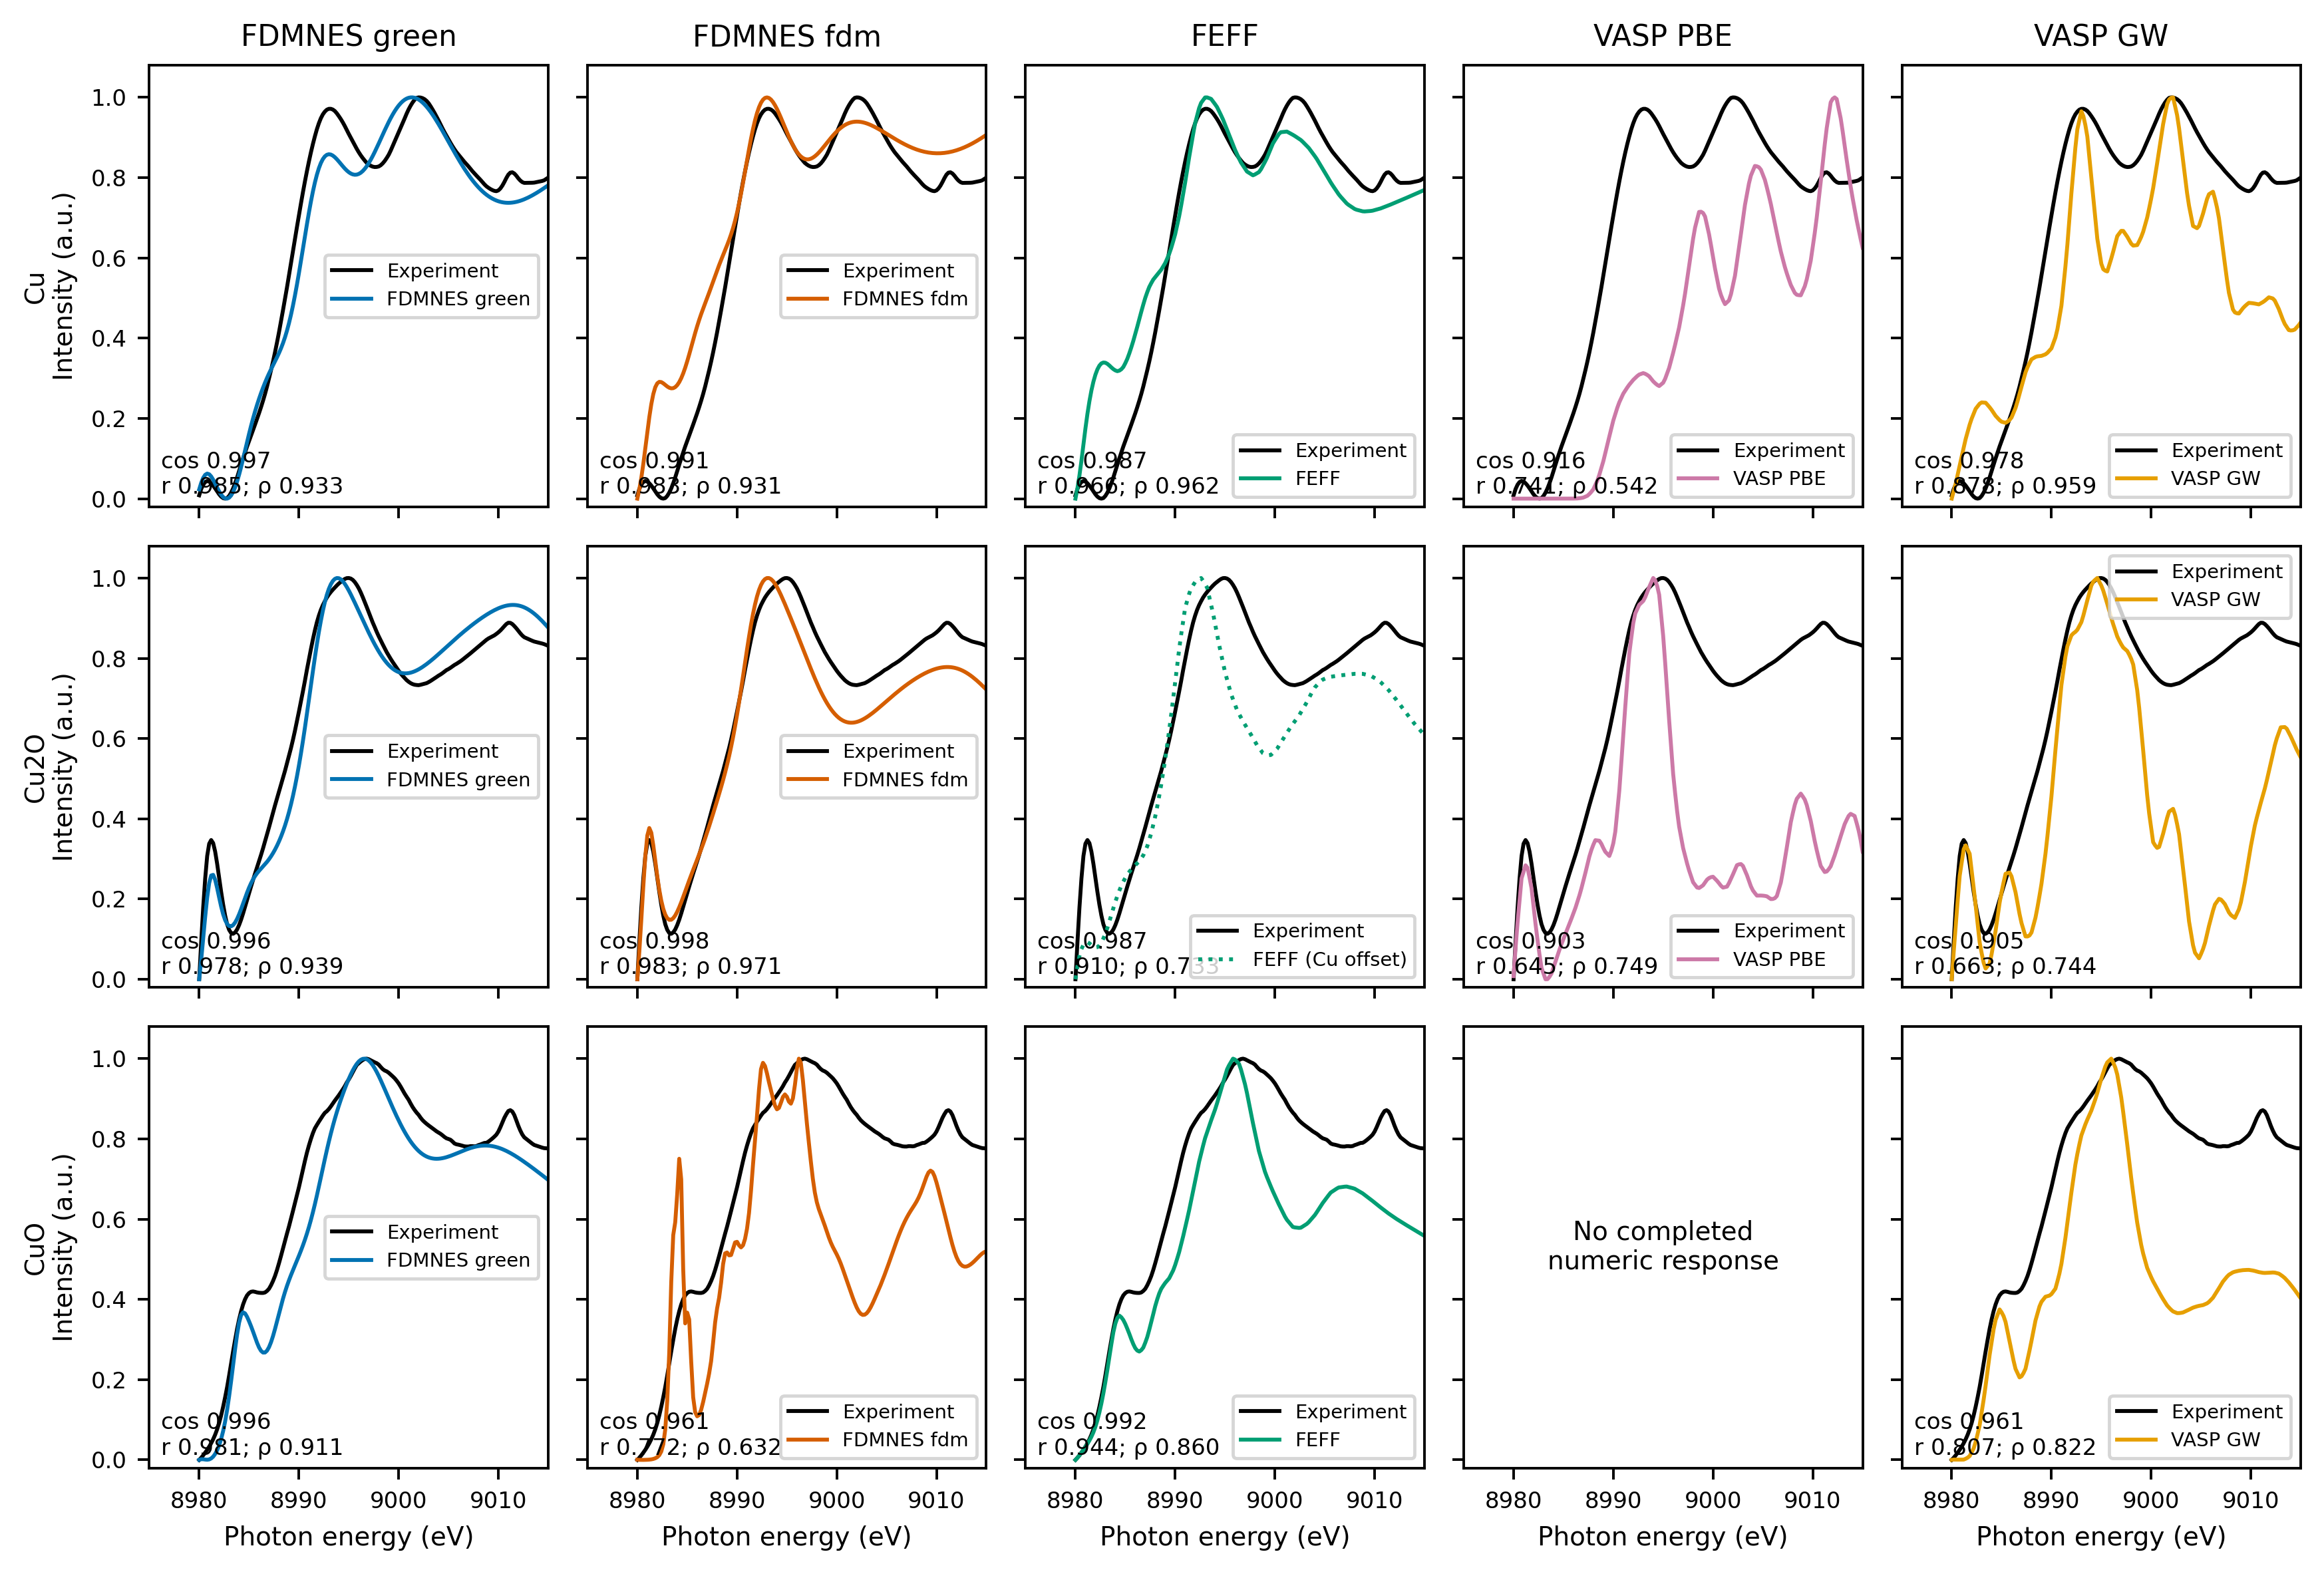
\includegraphics[width=\linewidth]{figures/SI_reference_grid.png}\caption{Three-material by five-method first-feature comparison, using actual numeric arrays and the same fixed min--max interval. Black denotes experiment. Missing CuO PBE is blank. The Cu$_2$O FEFF dotted trace is explicitly identified as retaining transferable Cu calibration.}\end{figure}
\begin{figure}[p]\centering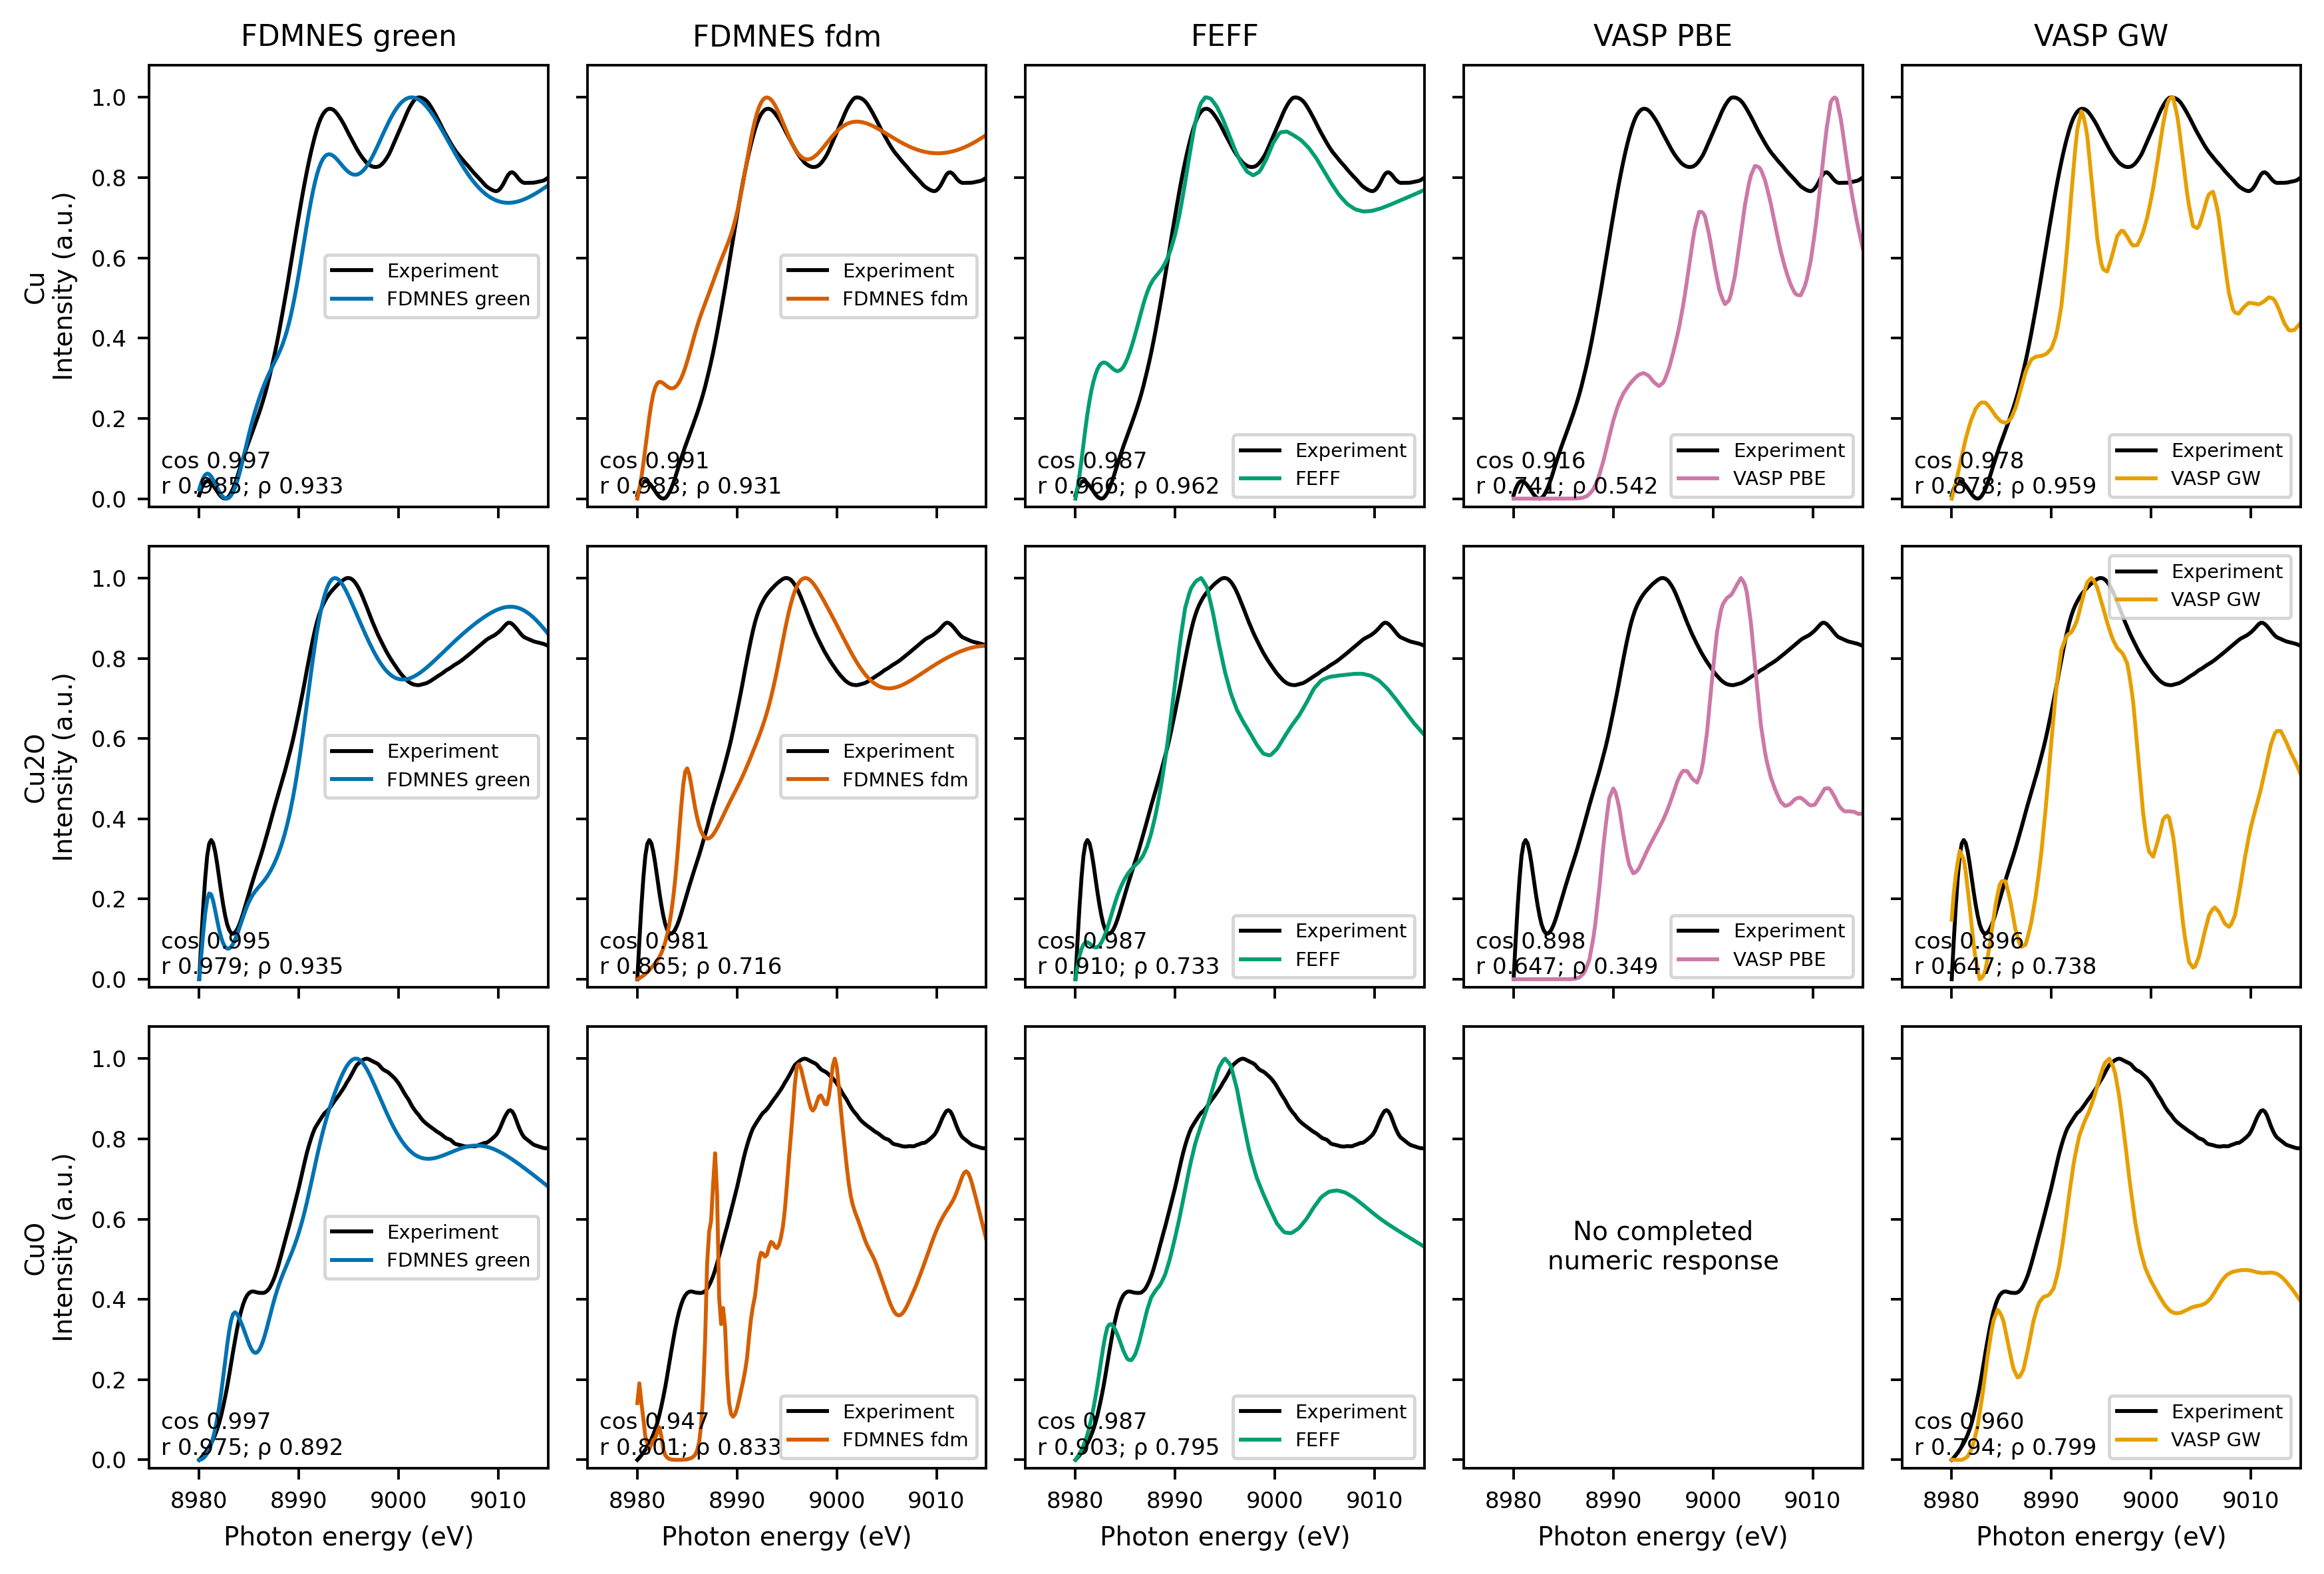
\includegraphics[width=\linewidth]{figures/SI_reference_Cu_calibrated.png}\caption{Transferable Cu-calibrated comparison, separately from first-feature shape alignment. Offsets are shared across compounds within each declared method, not forced to be shared between PBE and the GW-labelled dataset.}\end{figure}

The newly supplied Cu$_2$O OUTCAR and HDF5 arrays independently agree for 2000 energy points and diagonal tensor components. The isotropic signal is their diagonal average of the imaginary output component. Inputs specify PBE+$U$, $U_{eff}=6$ eV on Cu, ICORELEVEL=2, CLZ=1 and CH\_SIGMA=0.1 eV. Complete numeric table, electronic EDIFF convergence and normal termination footer are recorded separately; a complete table alone is not a convergence certificate. The CuO PBE HDF5 cannot be parsed (bad object-header version) and its supplied OUTCAR lacks a complete numeric table. Original files are uploaded with this limitation. PAW dataset labels and hashes are retained without licensed potential contents. GW-labelled PAW data do not establish a quasiparticle or electron--hole stage.

Timing provenance distinguishes measured CPU from allocated core-time estimates. CuO FDMNES fdm is retained as the author's corrected 129600 CPU s, with the older 91018.9 s archived log recorded separately rather than falsely identified as the same run. FEFF module values are CPU times. Cu$_2$O PBE SCF/XAS CPU times are 2400.813/7149.952 s; GW-labelled stages are 21585.344/8539.898 s. Resources, system sizes and settings differ, and no measured speedup is claimed. The complete timing CSV preserves stage and evidence distinctions.

\section{Current unfinished OCCO--water checkpoints}
Read-only snapshots were captured at 2026-10-27 01:45 UTC with source modification times and SHA-256. The actual current CONTCAR is used for identity; restart POSCAR need not be the original seed. Original dimer atoms are tracked element-wise with in-plane minimum images and nonperiodic vacuum. Connectivity is tested over C--C cutoffs 1.65--2.2~\AA, with explicit C--O and hydrogen graphs. Water hydrogen bonds are not covalent proton transfer. Two-C versus C,O binding is audited independently of C--C retention. The three captured current cases are all dissociated 2CO, not retained C2O2. Carbon flags are free in these checkpoints, rather than artificially fixed dimer bonds. Available restart-local trajectories do not establish a full history before the supplied restart.

\begin{center}\begin{tabular}{lrrrr}\toprule
Current case & Step & C--C/\AA & C--O/\AA & Free force/eV\,\AA$^{-1}$\\\midrule
2H$_2$O &16&3.283&1.159--1.165&0.288\\
2H$_2$O interior &1&3.105&1.166--1.167&0.280\\
2H$_2$O atop--bridge &8&3.476&1.163--1.182&0.291\\\bottomrule\end{tabular}\end{center}
All three are unfinished, without an ionic convergence message or covalent proton transfer to the original dimer. Last evaluated OUTCAR forces may correspond to the geometry before an optimizer-updated CONTCAR. Fifteen other seed-only alternatives are separately inventoried; their existence is not a running or completed relaxation. Current snapshots, available complete trajectories, OSZICAR and input/output evidence are retained. No snapshot is labeled a stable minimum or a completed training record.

\section{Reproducible shared inference and saved evidence}
A real local natural-language request calls the shared audited \texttt{differential\_v1} recipe: validate geometry-linked pairs, fit declared grouped recipes, save/reload, and infer held-out identity, loading and supported configuration-level geometry. One hundred main and forty geometry fold models are reloaded through the same feature API. Code/data hashes, split groups, missing-positive labels and preprocessing/reference conventions are stored. Scores are not asserted to be calibrated probabilities; unsupported chemistry/domain/reference queries are flagged or rejected. No production scheduler or newly generated spectrum is demonstrated.

Archived primary/fixed-winner reproduction remains separate from this current route. The primary and fixed winner match the recorded fresh arrays, 140/169 broader OOF files match, 29 differ, and five recorded fold-model reloads match. These historical results do not prove causation from dependency changes. Proposed missing controls and future configurations have not already improved inference.
\begin{thebibliography}{99}
\bibitem{ni2024} W. Ni, H. Chen, N. Tang \textit{et al.}, High-purity ethylene production via indirect carbon dioxide electrochemical reduction, \textit{Nat. Commun.}, 2024, \textbf{15}, 6078, DOI: \href{https://doi.org/10.1038/s41467-024-50522-7}{10.1038/s41467-024-50522-7}.
\bibitem{francis2018} S. A. Francis, J. M. Velazquez, I. M. Ferrer, D. A. Torelli, D. Guevarra, M. T. McDowell, K. Sun, X. Zhou, F. H. Saadi, J. John, M. H. Richter, F. P. Hyler, K. M. Papadantonakis, B. S. Brunschwig and N. S. Lewis, Reduction of aqueous CO\textsubscript{2} to 1-propanol at MoS\textsubscript{2} electrodes, \textit{Chem. Mater.}, 2018, \textbf{30}, 4902--4908, DOI: \href{https://doi.org/10.1021/acs.chemmater.7b04428}{10.1021/acs.chemmater.7b04428}.
\bibitem{zhan2024} C. Zhan, F. Dattila, C. Rettenmaier, A. Herzog, M. Herran, T. Wagner, F. Scholten, A. Bergmann, N. L\'opez and B. Roldan Cuenya, Key intermediates and Cu active sites for CO\textsubscript{2} electroreduction to ethylene and ethanol, \textit{Nat. Energy}, 2024, \textbf{9}, 1485--1496, DOI: \href{https://doi.org/10.1038/s41560-024-01633-4}{10.1038/s41560-024-01633-4}.
\bibitem{montoya2015} J. H. Montoya, C. Shi, K. Chan and J. K. N\o rskov, Theoretical insights into a CO dimerization mechanism in CO\textsubscript{2} electroreduction, \textit{J. Phys. Chem. Lett.}, 2015, \textbf{6}, 2032--2037, DOI: \href{https://doi.org/10.1021/acs.jpclett.5b00722}{10.1021/acs.jpclett.5b00722}.
\bibitem{operando2021} J. Timoshenko and B. Roldan Cuenya, In situ/operando electrocatalyst characterization by X-ray absorption spectroscopy, \textit{Chem. Rev.}, 2021, \textbf{121}, 882--961, DOI: \href{https://doi.org/10.1021/acs.chemrev.0c00396}{10.1021/acs.chemrev.0c00396}.
\bibitem{lin2020} S.-C. Lin, C.-C. Chang, S.-Y. Chiu, H.-T. Pai, T.-Y. Liao, C.-S. Hsu, W.-H. Chiang, M.-K. Tsai and H. M. Chen, Operando time-resolved X-ray absorption spectroscopy reveals the chemical nature enabling highly selective CO\textsubscript{2} reduction, \textit{Nat. Commun.}, 2020, \textbf{11}, 3525, DOI: \href{https://doi.org/10.1038/s41467-020-17231-3}{10.1038/s41467-020-17231-3}.
\bibitem{morales2018} C. G. Morales-Guio, E. R. Cave, S. A. Nitopi, J. T. Feaster, L. Wang, K. P. Kuhl, A. Jackson, N. C. Johnson, D. N. Abram, T. Hatsukade, C. Hahn and T. F. Jaramillo, Improved CO\textsubscript{2} reduction activity towards C\textsubscript{2+} alcohols on a tandem gold on copper electrocatalyst, \textit{Nat. Catal.}, 2018, \textbf{1}, 764--771, DOI: \href{https://doi.org/10.1038/s41929-018-0139-9}{10.1038/s41929-018-0139-9}.
\bibitem{rehr2010} J. J. Rehr, J. J. Kas, F. D. Vila, M. P. Prange and K. Jorissen, Parameter-free calculations of X-ray spectra with FEFF9, \textit{Phys. Chem. Chem. Phys.}, 2010, \textbf{12}, 5503--5513, DOI: \href{https://doi.org/10.1039/B926434E}{10.1039/B926434E}.
\bibitem{joly2001} Y. Joly, X-ray absorption near-edge structure calculations beyond the muffin-tin approximation, \textit{Phys. Rev. B}, 2001, \textbf{63}, 125120, DOI: \href{https://doi.org/10.1103/PhysRevB.63.125120}{10.1103/PhysRevB.63.125120}.
\bibitem{vasp1996} G. Kresse and J. Furthm\"uller, Efficient iterative schemes for ab initio total-energy calculations using a plane-wave basis set, \textit{Phys. Rev. B}, 1996, \textbf{54}, 11169--11186, DOI: \href{https://doi.org/10.1103/PhysRevB.54.11169}{10.1103/PhysRevB.54.11169}.
\bibitem{vaspxas} VASP Wiki, Supercell core-hole calculations, \url{https://vasp.at/wiki/index.php/SCH_calculations}, accessed 21 October 2026.
\bibitem{ocean2011} J. Vinson, J. J. Rehr, J. J. Kas and E. L. Shirley, Bethe--Salpeter equation calculations of core excitation spectra, \textit{Phys. Rev. B}, 2011, \textbf{83}, 115106, DOI: \href{https://doi.org/10.1103/PhysRevB.83.115106}{10.1103/PhysRevB.83.115106}.
\bibitem{timoshenko2018} J. Timoshenko, A. Anspoks, A. Cintins, A. Kuzmin, J. Purans and A. I. Frenkel, Neural network approach for characterizing structural transformations by X-ray absorption fine structure spectroscopy, \textit{Phys. Rev. Lett.}, 2018, \textbf{120}, 225502, DOI: \href{https://doi.org/10.1103/PhysRevLett.120.225502}{10.1103/PhysRevLett.120.225502}.
\bibitem{marcella2020} N. Marcella, Y. Liu, J. Timoshenko, E. Guan, M. Luneau, T. Shirman, A. M. Plonka, J. E. S. van der Hoeven, J. Aizenberg, C. M. Friend and A. I. Frenkel, Neural network assisted analysis of bimetallic nanocatalysts using X-ray absorption near edge structure spectroscopy, \textit{Phys. Chem. Chem. Phys.}, 2020, \textbf{22}, 18902--18910, DOI: \href{https://doi.org/10.1039/D0CP02098B}{10.1039/D0CP02098B}.
\bibitem{torrisi2020} S. B. Torrisi, M. R. Carbone, B. A. Rohr, J. H. Montoya, Y. Ha, J. Yano, S. K. Suram and L. Hung, Random forest machine learning models for interpretable X-ray absorption near-edge structure spectrum-property relationships, \textit{npj Comput. Mater.}, 2020, \textbf{6}, 109, DOI: \href{https://doi.org/10.1038/s41524-020-00376-6}{10.1038/s41524-020-00376-6}.
\bibitem{david2023} T. David, N. K. Nik Aznan, K. Garside and T. J. Penfold, Towards the automated extraction of structural information from X-ray absorption spectra, \textit{Digital Discovery}, 2023, \textbf{2}, 1461--1470, DOI: \href{https://doi.org/10.1039/D3DD00101F}{10.1039/D3DD00101F}.
\bibitem{chen2024} Y. Chen, C. Chen, I. Hwang, M. J. Davis, W. Yang, C. Sun, G.-H. Lee, D. McReynolds, D. Allan, J. Marulanda Arias, S. P. Ong and M. K. Y. Chan, Robust machine learning inference from X-ray absorption near edge spectra through featurization, \textit{Chem. Mater.}, 2024, \textbf{36}, 2304--2313, DOI: \href{https://doi.org/10.1021/acs.chemmater.3c02584}{10.1021/acs.chemmater.3c02584}.
\bibitem{jia2026} H. Jia, Y. Chen, G.-H. Lee, J. Smith, M. Chi, W. Yang and M. K. Y. Chan, Revealing local structures through machine-learning-fused multimodal spectroscopy, \textit{ACS Nano}, 2026, \textbf{20}, 4228--4240, DOI: \href{https://doi.org/10.1021/acsnano.5c16942}{10.1021/acsnano.5c16942}.
\bibitem{bran2024} A. M. Bran, S. Cox, O. Schilter, C. Baldassari, A. D. White and P. Schwaller, Augmenting large language models with chemistry tools, \textit{Nat. Mach. Intell.}, 2024, \textbf{6}, 525--535, DOI: \href{https://doi.org/10.1038/s42256-024-00832-8}{10.1038/s42256-024-00832-8}.
\bibitem{canty2023} R. B. Canty, B. A. Koscher, M. A. McDonald and K. F. Jensen, Integrating autonomy into automated research platforms, \textit{Digital Discovery}, 2023, \textbf{2}, 1259--1268, DOI: \href{https://doi.org/10.1039/D3DD00135K}{10.1039/D3DD00135K}.
\bibitem{vriza2026} A. Vriza \textit{et al.}, Multi-agentic AI framework for end-to-end atomistic simulations, \textit{Digital Discovery}, 2026, \textbf{5}, 440--452, DOI: \href{https://doi.org/10.1039/D5DD00435G}{10.1039/D5DD00435G}.
\bibitem{nersc} NERSC, The Superfacility API, \url{https://docs.nersc.gov/services/sfapi/}, accessed 21 October 2026.
\bibitem{fdmnesmanual} Y. Joly, \textit{FDMNES User's Guide}, November 2022, \url{https://data-analysis.synchrotron-soleil.fr/tmp/software/fdmnes/fdmnes_Linux/Doc/Manual_Eng.pdf}, accessed 21 October 2026.
\bibitem{ahmed1974} N. Ahmed, T. Natarajan and K. R. Rao, Discrete cosine transform, \textit{IEEE Trans. Comput.}, 1974, \textbf{C-23}, 90--93, DOI: \href{https://doi.org/10.1109/T-C.1974.223784}{10.1109/T-C.1974.223784}.
\bibitem{geurts2006} P. Geurts, D. Ernst and L. Wehenkel, Extremely randomized trees, \textit{Mach. Learn.}, 2006, \textbf{63}, 3--42, DOI: \href{https://doi.org/10.1007/s10994-006-6226-1}{10.1007/s10994-006-6226-1}.
\bibitem{montoya2013} J. H. Montoya, A. A. Peterson and J. K. N\o rskov, Insights into C--C coupling in CO\textsubscript{2} electroreduction on copper electrodes, \textit{ChemCatChem}, 2013, \textbf{5}, 737--742, DOI: \href{https://doi.org/10.1002/cctc.201200564}{10.1002/cctc.201200564}.
\bibitem{ramaker2010} D. E. Ramaker and D. C. Koningsberger, The atomic AXAFS and Delta mu XANES techniques as applied to heterogeneous catalysis and electrocatalysis, \textit{Phys. Chem. Chem. Phys.}, 2010, \textbf{12}, 5514--5534, DOI: \href{https://doi.org/10.1039/B927120C}{10.1039/B927120C}.
\bibitem{ramaker2014} D. E. Ramaker, A. Korovina, V. Croze, J. Melke and C. Roth, Following ORR intermediates adsorbed on a Pt cathode catalyst during break-in of a PEM fuel cell by in operando X-ray absorption spectroscopy, \textit{Phys. Chem. Chem. Phys.}, 2014, \textbf{16}, 13645--13653, DOI: \href{https://doi.org/10.1039/C4CP00192C}{10.1039/C4CP00192C}.
\end{thebibliography}

\end{document}
